\documentclass[11pt,a4paper]{article}
\usepackage[utf8]{inputenc}
\usepackage[T1]{fontenc}
\usepackage[margin=2.2cm]{geometry}
\usepackage{lmodern}
\usepackage{microtype}
\usepackage{amsmath,amssymb,bm}
\usepackage[table]{xcolor}
\usepackage{booktabs}
\usepackage{tabularx}
\usepackage{float}
\usepackage{graphicx}
\usepackage{enumitem}
\usepackage[most]{tcolorbox}
\usepackage{fancyhdr}
\usepackage{needspace}
\usepackage{titlesec}
\usepackage{tikz}
\usetikzlibrary{arrows.meta,positioning,calc,decorations.pathreplacing,shapes.geometric}
\usepackage[colorlinks=true,linkcolor=blue!60!black,urlcolor=blue!60!black]{hyperref}

\setlist[itemize]{nosep,leftmargin=*,topsep=2pt,partopsep=0pt}
\setlist[enumerate]{nosep,leftmargin=*,topsep=2pt,partopsep=0pt}
\widowpenalty=10000
\clubpenalty=10000
\setlength{\parskip}{0.55em}
\setlength{\parindent}{0pt}

\definecolor{cblue}{HTML}{2B6CB0}
\definecolor{cgreen}{HTML}{2F855A}
\definecolor{cred}{HTML}{C53030}
\definecolor{corange}{HTML}{DD6B20}
\definecolor{cgray}{HTML}{718096}
\definecolor{cpurple}{HTML}{6B46C1}

\titleformat{\section}{\Large\bfseries\color{cblue}}{\thesection}{0.6em}{}
\titleformat{\subsection}{\large\bfseries\color{cblue!80!black}}{\thesubsection}{0.6em}{}
\titleformat{\subsubsection}{\normalsize\bfseries\color{cblue!70!black}}{\thesubsubsection}{0.6em}{}

\pagestyle{fancy}
\fancyhf{}
\lhead{\small Paper 03 --- full explained guide}
\rhead{\small Achterhold et al., L4DC 2023}
\cfoot{\small\thepage}
\renewcommand{\headrulewidth}{0.3pt}

\newtcolorbox{idea}[1][]{colback=cblue!6,colframe=cblue!70,fonttitle=\bfseries,title={#1},boxrule=0.6pt,arc=2pt,left=6pt,right=6pt,top=4pt,bottom=4pt}
\newtcolorbox{toy}[1][]{colback=corange!7,colframe=corange!80,fonttitle=\bfseries,title={#1},boxrule=0.6pt,arc=2pt,left=6pt,right=6pt,top=4pt,bottom=4pt}
\newtcolorbox{warn}[1][]{colback=cred!6,colframe=cred!75,fonttitle=\bfseries,title={#1},boxrule=0.6pt,arc=2pt,left=6pt,right=6pt,top=4pt,bottom=4pt}
\newtcolorbox{eqbox}[1][]{colback=cgray!8,colframe=cgray!70,fonttitle=\bfseries,title={#1},boxrule=0.6pt,arc=2pt,left=6pt,right=6pt,top=4pt,bottom=4pt}
\newtcolorbox{ours}[1][]{colback=cgreen!6,colframe=cgreen!70,fonttitle=\bfseries,title={#1},boxrule=0.6pt,arc=2pt,left=6pt,right=6pt,top=4pt,bottom=4pt}

\newcommand{\vv}{\mathbf{v}}
\newcommand{\pp}{\mathbf{p}}
\newcommand{\zz}{\mathbf{z}}
\newcommand{\mm}{\mathbf{m}}
\newcommand{\ww}{\boldsymbol{\omega}}
\newcommand{\mmu}{\boldsymbol{\mu}}
\newcommand{\SSigma}{\boldsymbol{\Sigma}}
\newcommand{\splus}[1]{[#1]_+}

\begin{document}
\setcounter{tocdepth}{2}

\begin{center}
{\LARGE\bfseries\color{cblue} Paper 03 --- the complete explained guide}\\[0.6em]
{\large \textit{Black-Box vs.\ Gray-Box: A Case Study on Learning Table Tennis Ball Trajectory Prediction with Spin and Impacts}}\\[0.5em]
Jan Achterhold, Philip Tobuschat, Hao Ma, Dieter Buechler, Michael Muehlebach, Joerg Stueckler\\
Max Planck Institute for Intelligent Systems, T\"ubingen. Accepted at L4DC 2023. arXiv 2305.15189v2 (12 Jun 2023)\\[0.4em]
{\small Guide written 2026-10-31 for the ball-estimation chapter. Source: the paper PDF read in full (main text, 13 pages + supplement, 7 pages).}
\end{center}

\begin{idea}[How to read this guide]
Every section of the paper is explained in the same order as the paper, including the supplementary material.
Every symbol is explained when it first appears. Every number that comes from the paper is marked \textbf{(paper)}.
\begin{itemize}
\item \textbf{Blue boxes}: the main idea of a part.
\item \textbf{Grey boxes}: the paper's equations, written out and translated into words.
\item \textbf{Orange boxes (Toy example)}: numbers I invented to make an idea easy to see. They are \emph{not} from the paper.
\item \textbf{Red boxes}: my own critical comments (mistakes, gaps, things to check). They are not the authors' claims.
\item \textbf{Green boxes}: what the part means for \emph{our} MuJoCo project (2.5 m arena, static Panda arm, overhead depth camera).
\end{itemize}
If a part feels heavy, read only the blue boxes first, then come back.
\end{idea}

\begin{eqbox}[The paper in one box]
\textbf{Problem:} predict where a flying, spinning, bouncing table-tennis ball will be up to 1 s ahead, from noisy camera positions, so a robot can hit it.\\
\textbf{Method (gray-box):} an extended Kalman filter (EKF) whose motion model is real physics (gravity, air drag, Magnus/spin force, a bounce map),
whose unknown numbers (noise levels, starting uncertainties, bounce map, drag and spin constants, a small spin network) are \emph{learned} from recorded trajectories
by maximising how well the filter predicts each next measurement (the marginal log-likelihood).\\
\textbf{Results (paper):} better than two black-box neural networks (RSSM, TVAE) at every horizon from 0.1 to 1 s; using the launcher's settings to guess the initial spin
helps ``drastically''; median 1 s prediction error 10.3 cm on unseen launcher positions; a real muscle-driven robot returned 29 of 30 balls.
\end{eqbox}

\tableofcontents
\newpage

% =====================================================================
\section{The story in one page}
A robot that plays table tennis must know where the ball \emph{will be}, not where it is now. That is a \textbf{prediction} problem, and three things make it hard:
\begin{enumerate}
\item \textbf{Measurements are noisy and sometimes missing.} The cameras report a position that is always a little wrong, and sometimes they report nothing.
\item \textbf{The motion is curved.} Gravity pulls the ball down, the air slows it (drag), spin bends its path (Magnus effect), and the table bounce changes speed and spin suddenly.
\item \textbf{Some quantities cannot be seen.} The cameras see position only. Spin is invisible but changes the path and especially the bounce.
\end{enumerate}
The authors build a pipeline: \emph{camera positions $\rightarrow$ EKF with a physics model and learned numbers $\rightarrow$ best guess of position, velocity, spin $\rightarrow$ run the physics forward to predict.}

\begin{figure}[htbp]
\centering
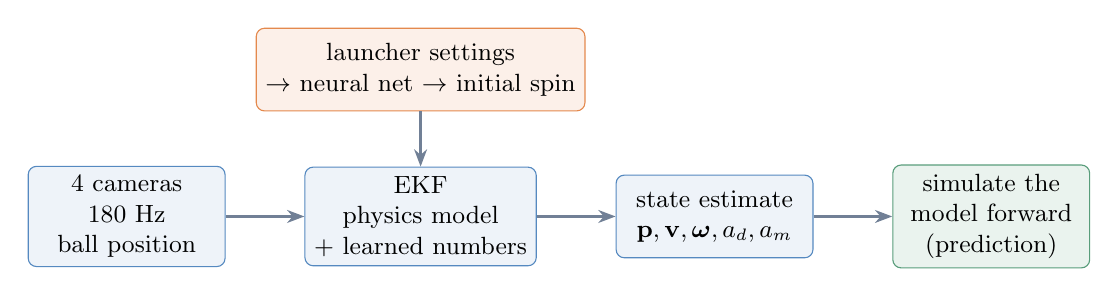
\begin{tikzpicture}[node distance=1.0cm,
  box/.style={draw=cblue!80,fill=cblue!8,rounded corners=3pt,minimum height=1.05cm,minimum width=2.5cm,align=center,font=\small},
  arr/.style={-{Stealth[length=2.2mm]},thick,cgray}]
\node[box] (cam) {4 cameras\\ 180 Hz\\ ball position};
\node[box,right=of cam] (filt) {EKF\\ physics model\\ + learned numbers};
\node[box,right=of filt] (state) {state estimate\\ $\pp,\vv,\ww,a_d,a_m$};
\node[box,right=of state,fill=cgreen!10,draw=cgreen!80] (pred) {simulate the\\ model forward\\ (prediction)};
\draw[arr] (cam) -- (filt); \draw[arr] (filt) -- (state); \draw[arr] (state) -- (pred);
\node[box,above=0.7cm of filt,fill=corange!10,draw=corange!80] (launch) {launcher settings\\ $\rightarrow$ neural net $\rightarrow$ initial spin};
\draw[arr] (launch) -- (filt);
\end{tikzpicture}
\caption{The pipeline of the paper. The robot re-plans its hitting point every time the estimate improves.}
\end{figure}

\paragraph{White, black and gray boxes.} A \textbf{white-box} model is pure physics (nothing learned). A \textbf{black-box} model is pure learning (a neural network that is told no physics).
A \textbf{gray-box} model keeps the physics \emph{structure} and learns only the numbers we do not know well. The paper's title asks: which is better for this problem? Its answer: gray-box.

% =====================================================================
\section{Background you need (explained from zero)}

\subsection{Vectors, norms and the cross product}
A \textbf{vector} is a list of numbers with a direction meaning, e.g.\ velocity $\vv=(v_x,v_y,v_z)$ in m/s. Its \textbf{norm} (length) is
$\|\vv\|=\sqrt{v_x^2+v_y^2+v_z^2}$, i.e.\ the speed. The \textbf{unit vector} $\hat\vv=\vv/\|\vv\|$ has length 1 and points the same way.

The \textbf{cross product} $\ww\times\vv$ of two 3D vectors is a third vector at a right angle to both:
\[
\ww\times\vv=\begin{pmatrix}\omega_y v_z-\omega_z v_y\\ \omega_z v_x-\omega_x v_z\\ \omega_x v_y-\omega_y v_x\end{pmatrix}
=\underbrace{\begin{pmatrix}0&-\omega_z&\omega_y\\ \omega_z&0&-\omega_x\\ -\omega_y&\omega_x&0\end{pmatrix}}_{[\ww]_\times}\vv .
\]
The matrix $[\ww]_\times$ (``skew matrix of $\ww$'') writes the cross product as a matrix times a vector. We need it later for derivatives.

\subsection{Gaussian (normal) distributions and covariance}
A \textbf{Gaussian} $\mathcal N(\mu,\sigma^2)$ is the bell curve with mean $\mu$ and variance $\sigma^2$ (standard deviation $\sigma$). About 68\% of draws fall within $\pm\sigma$, 95\% within $\pm2\sigma$.
For a vector, the bell curve is $\mathcal N(\mmu,\SSigma)$ with a mean vector $\mmu$ and a \textbf{covariance matrix} $\SSigma$: the diagonal holds the variance of each number, the off-diagonal entries say how two numbers vary together.
Its density at a point $\mathbf x\in\mathbb R^d$ is
\[
\mathcal N(\mathbf x;\mmu,\SSigma)=\frac{1}{\sqrt{(2\pi)^d\det\SSigma}}\exp\!\Big(-\tfrac12(\mathbf x-\mmu)^\top\SSigma^{-1}(\mathbf x-\mmu)\Big),
\]
\[
\log\mathcal N(\mathbf x;\mmu,\SSigma)=-\tfrac12\Big[(\mathbf x-\mmu)^\top\SSigma^{-1}(\mathbf x-\mmu)+\log\det\SSigma+d\log 2\pi\Big].
\]
\textbf{Read the log form slowly}, because the whole learning part of the paper is built on it: the first term is the \emph{squared surprise measured in units of the expected spread};
the second term \emph{punishes claiming a large spread}. So a model scores well only if it is \emph{both} close to the data \emph{and} honest-but-not-lazy about its uncertainty.
$\mathrm{diag}(\mathbf x)$ is the square matrix with $\mathbf x$ on the diagonal and zeros elsewhere.

\begin{toy}[Toy example (invented numbers) --- why both terms matter]
A measurement arrives 2 cm from the prediction (1D). Model A claimed $\sigma=1$ cm: surprise term $2^2/1^2=4$, spread term $\log 1=0$ $\Rightarrow$ score $-\tfrac12(4+0)=-2$ (ignoring the constant).
Model B claimed $\sigma=10$ cm: surprise $0.04$, spread $\log 100=4.6$ $\Rightarrow$ $-2.3$. Model C claimed $\sigma=2$ cm: surprise $1$, spread $\log 4=1.39$ $\Rightarrow$ $-1.19$, the best.
Over many measurements the best score goes to the model whose claimed $\sigma$ matches the real size of its errors.
\end{toy}

\subsection{Likelihood}
The \textbf{likelihood} of parameters $\Psi$ is ``how probable the observed data is if the parameters were $\Psi$''. Maximising it means choosing the parameters that make the data least surprising.
We use the logarithm because products of many probabilities become sums, which are numerically safe and easy to differentiate.

\subsection{Softplus: a trick to keep numbers positive}
Variances must be positive. Instead of constraining them, the paper stores an unconstrained number $x$ and uses
\[
\splus{x}=\log(1+e^x)+10^{-6}\quad\textbf{(paper)} .
\]
For large $x$, $\splus{x}\approx x$; for very negative $x$, $\splus{x}\to10^{-6}$. It is smooth and always positive. Its inverse, used to set starting values, is $\mathrm{inv}\splus{y}=\log(e^{y-10^{-6}}-1)$.

\subsection{Euler's method}
To simulate $\dot x=f(x)$ on a computer: $x(t+\Delta t)\approx x(t)+\Delta t\,f(x(t))$. Simple and fast; accurate when $\Delta t$ is small (here 5.56 ms).

\subsection{Jacobian}
For a function $\mathbf y=g(\mathbf x)$ from $\mathbb R^n$ to $\mathbb R^m$, the \textbf{Jacobian} $\mathbf J=\partial g/\partial\mathbf x$ is the $m\times n$ table of partial derivatives: entry $(i,j)$ says how much $y_i$ changes when $x_j$ changes a tiny bit.
It is the best straight-line (linear) approximation of $g$ near a point.

\subsection{Kalman filter and extended Kalman filter}
A \textbf{Kalman filter} keeps a Gaussian belief $\mathcal N(\mmu,\SSigma)$ about the state and repeats two steps:
\begin{itemize}
\item \textbf{Predict} with the model: the mean moves forward, the uncertainty grows (model imperfect, process noise $\mathbf Q$).
\item \textbf{Correct} with a measurement: move the mean towards the measurement by a weight $\mathbf K$ (Kalman gain) that depends on how uncertain the prediction and the measurement (noise $\mathbf R$) are.
\end{itemize}
It is exact for linear models with Gaussian noise. The \textbf{EKF} handles a curved model by using its Jacobian to carry the covariance through each step.

\begin{toy}[Toy example (invented numbers) --- one correction in 1D]
Prediction $101.1\pm4$ cm (variance 16), camera $106\pm3$ cm (variance 9). Gain $K=16/(16+9)=0.64$. New estimate $101.1+0.64(106-101.1)=104.2$ cm, variance $(1-0.64)\cdot16=5.76$, i.e.\ $\pm2.4$ cm.
The blend is more certain than either source.
\end{toy}

% =====================================================================
\section{Paper Section 1 --- Introduction: what they claim}
The authors state three contributions \textbf{(paper)}:
\begin{enumerate}
\item A \textbf{gray-box} EKF for table-tennis balls with a physical model (drag, spin, impacts) whose parameters are \emph{trained from offline data}; it predicts better than two deep-learning (black-box) baselines.
\item \textbf{Estimating the initial spin from the ball launcher's parameters} with a neural network ``drastically'' improves prediction over an uninformed spin start.
\item A real-robot test: a pneumatic artificial-muscle arm \textbf{returns balls} using the predictions.
\end{enumerate}

% =====================================================================
\section{Paper Section 2 --- Related work, explained}
\subsection{Three model classes}
\begin{itemize}
\item \textbf{Black box}: statistical, data only. Typical form: an \emph{encoder} maps observations into a hidden (latent) space, a \emph{forward model} steps the latent state in time, a \emph{decoder} maps back.
Forward models are often recurrent networks: \textbf{LSTM} and \textbf{GRU}. Adding random (stochastic) nodes gives \textbf{VRNN}, \textbf{SRNN}. Models that do filtering in latent space: \textbf{Kalman-VAE}, \textbf{Recurrent Kalman Networks}, \textbf{Deep Variational Bayes Filters}.
\textbf{RSSM} (Hafner et al.\ 2019, recurrent state-space model, used for model-based reinforcement learning) is one of the two baselines.
\item \textbf{White box}: prior knowledge only, no data.
\item \textbf{Gray box}: physics structure + data. One line of work is \textbf{differentiable physics engines} (gradients through a simulator for system identification).
``System identification'' is the classic name for fitting dynamic models to data (Ljung 1986).
\end{itemize}
\subsection{Table tennis trajectory modelling}
\begin{itemize}
\item White-box: aerodynamic model (gravity, drag, Magnus) + physics-based rebound model inside an EKF or UKF (many works cited).
\item Black-box: polynomial curves fitted to recorded data; and the deep conditional generative model \textbf{TVAE} of G\'omez-Gonz\'alez et al.\ (2020), the second baseline.
\item The spin problem: spin is hard to infer from positions. Earlier works watched the \textbf{brand logo} on the ball or put an \textbf{inertial sensor in the racket}. This paper instead uses the \textbf{launcher's settings}.
\end{itemize}

% =====================================================================
\section{Paper Section 3.1 --- The physical model}
\subsection{Free flight (Eq.~1)}
\begin{eqbox}[Equation 1 (paper)]
\[
\dot\vv(t)=-k_d\,\|\vv(t)\|_2\,\vv(t)+k_m\,\big(\ww(t)\times\vv(t)\big)+\mathbf g,\qquad \mathbf g=(0,0,-9.802)^\top\ \text{m/s}^2 .
\]
\textbf{Words:} acceleration = air drag + spin (Magnus) force + gravity.
\begin{itemize}
\item $-k_d\|\vv\|\vv$: \emph{drag}. Its size is $k_d\|\vv\|^2$ (quadratic in speed), its direction is opposite to the motion. $k_d$ [1/m] says how strongly the air brakes this ball.
\item $k_m(\ww\times\vv)$: \emph{Magnus force}. $\ww$ is the spin (angular velocity, rad/s). The force is perpendicular to both the spin axis and the velocity, which is why topspin makes the ball dip and sidespin curves it. $k_m$ (dimensionless) says how strong this is.
\item $\mathbf g$: gravity, $z$ axis up, value 9.802 m/s$^2$ \textbf{(paper)}.
\end{itemize}
\end{eqbox}
\paragraph{Where the constants come from physically.} In aerodynamics $k_d=C_d\rho A/(2m)$ with drag coefficient $C_d$, air density $\rho$, cross-section $A=\pi r^2$, mass $m$.
The paper gives the analogous formula for the Magnus constant, $k_m^*=C_m\rho A r/(2m)$ (Section 4.3). In the paper these constants are \emph{learned}, not computed.

\begin{toy}[Toy example (invented numbers) --- sizes of the three terms]
Take $k_d=0.1$ /m, speed 5 m/s: drag $=0.1\cdot5^2=2.5$ m/s$^2$. Gravity 9.8 m/s$^2$. If $k_m=0.05$ and the spin is 50 rad/s at right angles to $\vv$, Magnus $=0.05\cdot50\cdot5=12.5$ m/s$^2$ --- as big as gravity.
That is why spin matters so much in table tennis.
\end{toy}

\subsection{The table impact (Eq.~2)}
\begin{eqbox}[Equation 2 (paper)]
\[
\begin{pmatrix}\vv^+\\ \ww^+\end{pmatrix}=\mathbf C\begin{pmatrix}\vv^-\\ \ww^-\end{pmatrix},\qquad\mathbf C\in\mathbb R^{6\times6}.
\]
\textbf{Words:} the 6 numbers just after the bounce ($+$) are a fixed linear mix of the 6 numbers just before ($-$). $\mathbf C$ is learned from data, not derived.
\end{eqbox}
A real impact involves friction, slipping and rolling and is nonlinear. A linear map is the simplest model that can still let spin change the outgoing velocity (and velocity change the spin).

% =====================================================================
\section{Paper Section 3.2 --- Discrete-time state-space model}
\subsection{The state (Eq.~3)}
\[
\zz(t)=(\pp^\top,\ \vv^\top,\ \ww^\top,\ a_d,\ a_m)^\top\in\mathbb R^{11},\qquad k_d=a_d^2+\epsilon,\quad k_m=a_m^2+\epsilon,\quad\epsilon=0.05\ \textbf{(paper)}.
\]
\begin{itemize}
\item $\pp$: ball centre position (3), $\vv$: velocity (3), $\ww$: spin (3), and two helper numbers $a_d,a_m$ for the air constants.
\item \textbf{Key idea:} the physics constants are \emph{inside the state}. The filter therefore estimates them while the ball flies, separately for each ball.
\item Squaring keeps $k_d,k_m\geq\epsilon>0$ without constraints; $\epsilon$ keeps them away from zero and ``stabilises training'' \textbf{(paper)}.
\end{itemize}

\subsection{Free-flight step (Eq.~4)}
Euler discretisation of Eq.~1 over a time $\Delta_t$:
\begin{eqbox}[Equation 4 (paper)]
\[
\begin{aligned}
\pp(t+\Delta_t)&=\pp(t)+\Delta_t\,\vv(t)\\
\vv(t+\Delta_t)&=\vv(t)+\Delta_t\big(-k_d(t)\|\vv(t)\|\vv(t)+k_m(t)(\ww(t)\times\vv(t))+\mathbf g\big)\\
\ww(t+\Delta_t)&=\ww(t),\qquad a_d(t+\Delta_t)=a_d(t),\qquad a_m(t+\Delta_t)=a_m(t).
\end{aligned}
\]
\end{eqbox}
The whole step is written $\zz(t+\Delta_t)=g_{\text{free}}(\zz(t),\Delta_t)$. Spin and the air constants do not change in free flight (only through process noise in the filter, see Eq.~6).
The camera period is $\Delta T=1/180$ s $\approx5.56$ ms \textbf{(paper)} because the four cameras are triggered at 180 Hz. With index $n$: $\zz_{n+1}=g_{\text{free}}(\zz_n,\Delta T)$.

\subsection{Impact inside a step}
An impact happens between $n$ and $n+1$ if the lowest point of the ball goes below the table: $p_{z,n+1}-r<z_{\text{table}}$ ($r$ = ball radius).
The time of impact $\Delta_{\text{imp}}\in[0,\Delta T]$ is approximated with \textbf{gravity only} (``a simplified model to avoid numerical instabilities'', paper):
\begin{eqbox}[Impact time (paper)]
\[
\Delta_{\text{imp}}=-\Big(v_{z,n}+\sqrt{v_{z,n}^2+2g_z h}\Big)\Big/g_z,\qquad h=-\big((p_{z,n}-r)-z_{\text{table}}\big),\quad g_z=-9.802 .
\]
\end{eqbox}
\textbf{Derivation (mine, to check the formula).} Let $h'=(p_{z,n}-r)-z_{\text{table}}>0$ be the gap above the table. Under gravity only, the gap after time $t$ is $h'+v_{z,n}t+\tfrac12 g_z t^2$.
Setting it to zero: $t=\big(-v_{z,n}\pm\sqrt{v_{z,n}^2-2g_zh'}\big)/g_z$. Because $g_z<0$, the positive root uses the minus sign: $t=-\big(v_{z,n}+\sqrt{v_{z,n}^2-2g_zh'}\big)/g_z$.
With $h=-h'$, $-2g_zh'=2g_zh$, which is exactly the paper's formula. \checkmark

\begin{toy}[Toy example (invented numbers) --- locating a bounce]
$v_z=-3$ m/s, gap $h'=1$ cm. $\sqrt{9+2\cdot9.802\cdot0.01}=\sqrt{9.196}=3.0325$. $\Delta_{\text{imp}}=-(-3+3.0325)/(-9.802)=0.0033$ s $=3.3$ ms $<5.56$ ms: the impact is inside the step.
\end{toy}

Inside the step: (1) fly $\Delta_{\text{imp}}$ to get $\zz^-=g_{\text{free}}(\zz_n,\Delta_{\text{imp}})$; (2) apply the impact $\zz^+=\mathbf C'\zz^-$ with $\mathbf C'=\mathrm{blockdiag}(\mathbf I_3,\mathbf C,1,1)$ (position and air constants unchanged, velocity and spin mapped by $\mathbf C$);
(3) fly the rest $\Delta T-\Delta_{\text{imp}}$.

\begin{figure}[htbp]
\centering
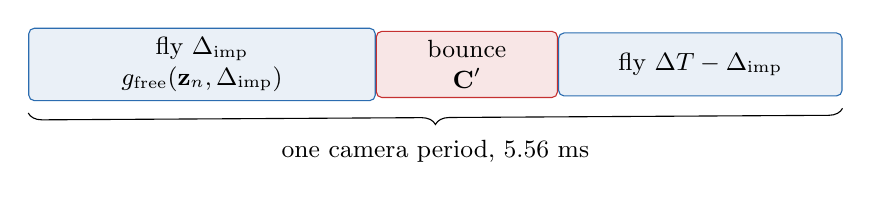
\begin{tikzpicture}[seg/.style={draw,rounded corners=2pt,minimum height=0.8cm,font=\small,align=center}]
\node[seg,fill=cblue!10,draw=cblue,minimum width=4.4cm] (a) at (0,0) {fly $\Delta_{\text{imp}}$\\ $g_{\text{free}}(\zz_n,\Delta_{\text{imp}})$};
\node[seg,fill=cred!12,draw=cred,minimum width=2.3cm,right=0cm of a] (b) {bounce\\ $\mathbf C'$};
\node[seg,fill=cblue!10,draw=cblue,minimum width=3.6cm,right=0cm of b] (c) {fly $\Delta T-\Delta_{\text{imp}}$};
\draw[decorate,decoration={brace,amplitude=5pt,mirror}] ($(a.south west)+(0,-0.15)$) -- ($(c.south east)+(0,-0.15)$) node[midway,below=7pt,font=\small] {one camera period, 5.56 ms};
\end{tikzpicture}
\caption{One step that contains a bounce.}
\end{figure}

\subsection{The joint model (Eq.~5)}
\begin{eqbox}[Equation 5 (paper)]
\[
\zz_{n+1}=g(\zz_n)=\begin{cases}g_{\text{free}}(\zz_n,\Delta T) & \text{if }[g_{\text{free}}(\zz_n,\Delta T)]_z-r\geq z_{\text{table}}\\[2pt]
g_{\text{free}}\big(\mathbf C'g_{\text{free}}(\zz_n,\Delta_{\text{imp}}),\ \Delta T-\Delta_{\text{imp}}\big) & \text{otherwise.}\end{cases}
\]
$[\zz]_z$ takes the $z$ coordinate of the position.
\end{eqbox}

\begin{ours}[For our project]
Our ball is planar, so there is no gravity, drag or Magnus in the plane. The free-flight part becomes \emph{sliding friction}: $\dot\vv=-\mu\,\hat\vv$ (constant deceleration $\mu$ opposite to the motion),
which is what \texttt{estimators/model.py} does. Our ``impact'' is a wall or arm-box bounce with restitution $E$; the normal velocity is multiplied by $-E$. Instead of an analytic impact time, we mirror the
overshoot (walls) or use a swept segment test (arm box). The idea ``constants in the state'' maps to putting $\mu$ (and later $E$) in our state.
\end{ours}

% =====================================================================
\section{Paper Section 3.3 --- The extended Kalman filter}
\subsection{Noise model (Eq.~6) and measurements}
\begin{eqbox}[Equation 6 and the measurement model (paper)]
\[
\hat\zz_{n+1}=g(\hat\zz_n)+\boldsymbol\zeta,\qquad\boldsymbol\zeta\sim\mathcal N\big(\mathbf 0,\ \mathrm{diag}(\splus{\boldsymbol\sigma_q})\big),\ \boldsymbol\sigma_q\in\mathbb R^{11};
\]
\[
\mm_n=\hat\pp_n+\boldsymbol\epsilon,\qquad\boldsymbol\epsilon\sim\mathcal N\big(\mathbf 0,\ \mathrm{diag}(\splus{\boldsymbol\sigma_r})\big),\ \boldsymbol\sigma_r\in\mathbb R^3 .
\]
\end{eqbox}
So $\mathbf Q=\mathrm{diag}(\splus{\boldsymbol\sigma_q})$ (one variance per state number, 11 values) and $\mathbf R=\mathrm{diag}(\splus{\boldsymbol\sigma_r})$ (one variance per axis).
Note that $\splus{\cdot}$ gives the \emph{variance} directly (not the standard deviation). Process noise on $\ww,a_d,a_m$ is what lets the filter slowly change spin and the air constants.

\subsection{Missing measurements: the operator $\tau(n)$}
The tracker sometimes returns nothing (e.g.\ occlusion). $\tau(n)$ is the time index of the $n$-th \emph{available} measurement. During a gap the filter does several predict steps and corrects only at the next available measurement.

\subsection{Predict and correct}
\begin{eqbox}[Predict (paper)]
\[
\mmu_{n+1|1:n}=g(\mmu_{n|1:n}),\qquad\SSigma_{n+1|1:n}=\mathbf J\SSigma_{n|1:n}\mathbf J^\top+\mathbf Q,\qquad\mathbf J=\frac{\partial g(\zz_n)}{\partial\zz_n}\Big|_{\zz_n=\mmu_{n|1:n}} .
\]
\end{eqbox}
The subscript ``$n+1|1:n$'' reads ``belief at time $n+1$ given measurements 1 to $n$''.
\begin{eqbox}[Correct (paper)]
\[
\mathbf H=[\mathbf I_3,\ \mathbf 0_{3\times8}],\qquad\mathbf K=\SSigma_{n+1|1:n}\mathbf H^\top\big(\mathbf H\SSigma_{n+1|1:n}\mathbf H^\top+\mathbf R\big)^{-1},
\]
\[
\mmu_{n+1|1:n+1}=\mmu_{n+1|1:n}+\mathbf K\big(\mm_{n+1}-\mathbf H\mmu_{n+1|1:n}\big),\qquad\SSigma_{n+1|1:n+1}=(\mathbf I-\mathbf K\mathbf H)\SSigma_{n+1|1:n}.
\]
\end{eqbox}
\begin{itemize}
\item $\mathbf H$ picks the position out of the 11-number state: the camera sees position only.
\item $\mathbf S=\mathbf H\SSigma\mathbf H^\top+\mathbf R$ ($3\times3$) is the \emph{innovation covariance}: how spread the next measurement is expected to be.
\item $\mm-\mathbf H\mmu$ is the \emph{innovation} (surprise). $\mathbf K$ ($11\times3$) decides how much each of the 11 numbers moves because of the surprise.
\end{itemize}
\paragraph{How spin and $a_d$ get corrected although they are never measured.} The covariance $\SSigma$ links them to position: e.g.\ a larger $a_d$ would have made the ball slower, hence at a different position.
When the measured position differs, $\mathbf K$ distributes the correction to $a_d$ (and spin) through these links. This is the essential mechanism we want for $\mu$.

\subsection{State initialisation}
The filter starts at the \textbf{second available measurement}:
\begin{itemize}
\item position mean $\pp=\mm_{\tau(2)}$; velocity mean by finite difference $\vv=(\mm_{\tau(2)}-\mm_{\tau(1)})/(\Delta T(\tau(2)-\tau(1)))$;
\item position and velocity covariances are \emph{learned}: $\SSigma_p=\mathrm{diag}(\splus{\boldsymbol\sigma_p})$, $\SSigma_v=\mathrm{diag}(\splus{\boldsymbol\sigma_v})$;
\item $a_d,a_m$: learned mean and learned variances $\splus{\sigma_{a_d}},\splus{\sigma_{a_m}}$;
\item spin: from the launcher (next subsection), or after an impact $\ww=\mathbf 0$ with learned variance $\mathrm{diag}(\splus{\boldsymbol\sigma_{\omega,\text{ai}}})$.
\end{itemize}
Full initial belief: $\mmu=(\pp^\top,\vv^\top,\ww^\top,a_d,a_m)^\top$, $\SSigma=\mathrm{blockdiag}(\SSigma_p,\SSigma_v,\SSigma_\omega,\splus{\sigma_{a_d}},\splus{\sigma_{a_m}})$.

\subsection{Spin from the launcher}
\begin{figure}[htbp]
\centering
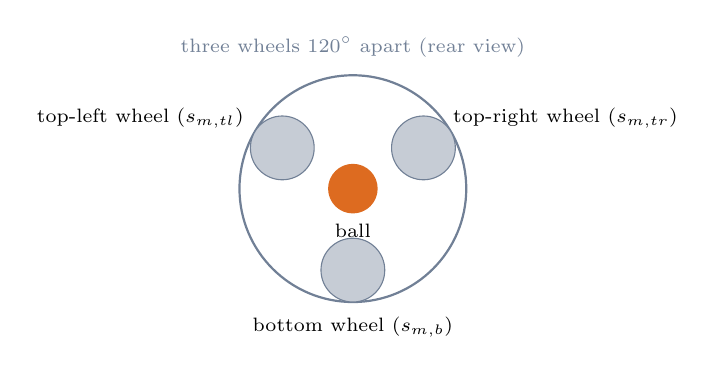
\begin{tikzpicture}[scale=0.9]
\draw[thick,cgray] (0,0) circle (1.6);
\fill[corange] (0,0) circle (0.35); \node[font=\scriptsize] at (0,-0.6) {ball};
\fill[cgray!40,draw=cgray] (0,-1.15) circle (0.45); \node[font=\scriptsize] at (0,-1.95) {bottom wheel ($s_{m,b}$)};
\fill[cgray!40,draw=cgray] ({1.15*cos(30)},{1.15*sin(30)}) circle (0.45); \node[font=\scriptsize,align=left] at (3.0,1.0) {top-right wheel ($s_{m,tr}$)};
\fill[cgray!40,draw=cgray] ({-1.15*cos(30)},{1.15*sin(30)}) circle (0.45); \node[font=\scriptsize,align=right] at (-3.0,1.0) {top-left wheel ($s_{m,tl}$)};
\node[font=\scriptsize,cgray] at (0,2.0) {three wheels 120$^\circ$ apart (rear view)};
\end{tikzpicture}
\caption{The launcher (drawing after the paper's Fig.~3b): three rubber wheels driven by brushless motors. Different wheel speeds give the ball speed and spin.}
\end{figure}
The launcher has 5 settings in $[0,1]$: three motor actuations $\mathbf s_m=(s_{m,tl},s_{m,tr},s_{m,b})$ and two aiming settings $s_\phi$ (azimuth), $s_\theta$ (elevation) \textbf{(paper)}.
\begin{enumerate}
\item A neural network $f^\omega(\mathbf s_m,\psi_f)$ predicts a \textbf{canonical spin} $\ww_{\rightarrow x}$ for a launcher shooting along the $x$ axis, and $f^{\Sigma\omega}$ its variances. Architecture (supplement S.3.3):
$\mathbf w_{\rightarrow x,\mu,\sigma}=\mathbf W_2\max(\mathbf W_1\mathbf s_m,0)$ with $\mathbf W_1\in\mathbb R^{256\times3}$, $\mathbf W_2\in\mathbb R^{6\times256}$: one hidden layer of 256 ReLU units, 6 outputs (3 means, 3 variances through softplus). No bias terms are written.
\item The canonical spin is rotated into the world: $\ww=\mathbf R_{\text{rot}}\ww_{\rightarrow x}$, $\SSigma_\omega=\mathbf R_{\text{rot}}\SSigma_{\omega\rightarrow x}\mathbf R_{\text{rot}}^\top$, with $\mathbf R_{\text{rot}}(\phi_f+\phi_l,\theta_l)$.
Angles: $\phi_f$ = rotation of the whole launcher frame about $z$; $\phi_l$, $\theta_l$ = azimuth and elevation of the launcher head.
\item $\phi_l,\theta_l$ come from \textbf{piecewise linear regressions} $s_\phi\mapsto\phi_l$, $s_\theta\mapsto\theta_l$ fitted on the training split of the default orientation (Fig.~4; one outlier excluded).
Default orientation: shooting along $-y$, i.e.\ $\phi_f=-90^\circ$. In simulation / on the robot they \emph{infer} $\phi_f+\phi_l$ from the first two measurements instead of measuring $\phi_f$.
\item An indicator $\mathbb 1_{\text{ai}}$ says whether $\mm_{\tau(2)}$ is after an impact. If yes, the launcher relation no longer holds: $\ww=\mathbf 0$, $\SSigma_\omega=\mathrm{diag}(\splus{\boldsymbol\sigma_{\omega,\text{ai}}})$.
\item Information given to the model: $(\phi_f,\phi_l,\theta_l,\mathbf s_m,\mathbb 1_{\text{ai}})$. \textbf{Ablation} without launch info: $\ww=\mathbf 0$, $\SSigma_\omega=\mathrm{diag}(\splus{\boldsymbol\sigma_\omega})$.
\end{enumerate}

\subsection{The learned parameter set}
\[
\Psi=\{\mathbf C,\ \boldsymbol\sigma_q,\ \boldsymbol\sigma_r,\ \boldsymbol\sigma_p,\ \boldsymbol\sigma_v,\ \psi_f,\ \boldsymbol\sigma_\omega,\ \boldsymbol\sigma_{\omega,\text{ai}},\ a_d,\ a_m,\ \sigma_{a_d},\ \sigma_{a_m}\}\quad\textbf{(paper)}.
\]
\begin{table}[htbp]
\centering\small\renewcommand{\arraystretch}{1.2}
\begin{tabularx}{\textwidth}{@{}l c X@{}}
\toprule
Symbol & count & Meaning \\
\midrule
$\mathbf C$ & 36 & bounce map \\
$\boldsymbol\sigma_q$ & 11 & process noise variances (per state number) \\
$\boldsymbol\sigma_r$ & 3 & camera noise variances \\
$\boldsymbol\sigma_p,\boldsymbol\sigma_v$ & 3+3 & initial position / velocity variances \\
$\psi_f$ & $\approx$2.3k & spin network weights ($256\cdot3+6\cdot256=2304$) \\
$\boldsymbol\sigma_\omega,\boldsymbol\sigma_{\omega,\text{ai}}$ & 3+3 & initial spin variances (no launch info / after impact) \\
$a_d,a_m,\sigma_{a_d},\sigma_{a_m}$ & 4 & initial means and variances of the air constants \\
\bottomrule
\end{tabularx}
\caption{What is learned. Apart from the network, it is only about 70 numbers (the counts are my own, from the shapes in the paper).}
\end{table}

% =====================================================================
\section{Paper Section 3.3 (end) --- Learning the filter}
\subsection{The objective (Eq.~7)}
Training data: $K$ recorded trajectories of positions. Each is cut into overlapping \textbf{chunks} of $N=50$ consecutive measurements:
a trajectory of length $L$ gives $L+1-N$ chunks $(\mm_i,\dots,\mm_{i+N-1})$. Chunks are drawn uniformly. The parameters maximise the expected log-likelihood
\[
\max_\Psi\ \mathbb E_{\mm_{1:N}\sim\Delta(P_c)}\ \log p(\mm_{3:N}\mid\mm_1,\mm_2,\Psi).
\]
\begin{eqbox}[Equation 7 (paper) --- prediction-error decomposition]
\[
\log p(\mm_{3:N}\mid\mm_1,\mm_2,\Psi)=\sum_{n=3}^N\log p(\mm_n\mid\mm_{1:n-1},\Psi)=\sum_{n=3}^N\log\mathcal N\big(\mm_n;\ \mmu_{n|1:n-1},\ \SSigma_{n|1:n-1}\big).
\]
\textbf{Words:} the probability of a whole chunk is the product of ``probability of each measurement given all earlier ones''. The EKF provides exactly these one-step-ahead predictions, so the score is computed in one pass, cost $O(N)$ (Särkkä 2013).
\end{eqbox}
\paragraph{What exactly is inside $\mathcal N(\cdot)$.} The measurement has 3 numbers but $\mmu,\SSigma$ are for 11. The predictive distribution of the next measurement is, by the measurement model,
\[
p(\mm_n\mid\mm_{1:n-1})=\mathcal N\big(\mm_n;\ \mathbf H\mmu_{n|1:n-1},\ \mathbf S_n\big),\qquad\mathbf S_n=\mathbf H\SSigma_{n|1:n-1}\mathbf H^\top+\mathbf R .
\]
Writing the log density out (Section 2.2), one chunk scores
\[
\sum_{n=3}^N-\tfrac12\Big[\mathbf y_n^\top\mathbf S_n^{-1}\mathbf y_n+\log\det\mathbf S_n+3\log2\pi\Big],\qquad\mathbf y_n=\mm_n-\mathbf H\mmu_{n|1:n-1}.
\]
\begin{warn}[My comment: notation shortcut]
The paper writes $\mathcal N(\mm_n;\mmu_{n|1:n-1},\SSigma_{n|1:n-1})$, mixing an 11-dim mean with a 3-dim measurement. The meaning must be the projected form above ($\mathbf H\mmu$, $\mathbf S=\mathbf H\SSigma\mathbf H^\top+\mathbf R$) --- that is the standard result in Särkkä (2013), which they cite.
If you implement it, use $\mathbf S$ including $\mathbf R$, otherwise $\mathbf R$ would never be learned.
\end{warn}
\paragraph{Why condition on the first two measurements?} They are used to start the filter (position and finite-difference velocity), so they cannot also be ``predicted''. The goal is a good filter/predictor, not a generative model of whole chunks.
\paragraph{Why chunks of 50?} Cheap passes (each chunk costs 50 filter steps), many different starting moments (the filter must work from any start), and mini-batches for stochastic optimisation.
\paragraph{Optimiser.} Adam, learning rate $5\cdot10^{-3}$, batch of 64 chunks \textbf{(paper)}. Gradients of the score with respect to $\Psi$ flow back through every filter step, because every step (including the Jacobians, see Section~\ref{sec:jac}) is made of differentiable operations.

\begin{toy}[Toy example (invented numbers) --- how learning finds $\mathbf R$]
If the filter assumes camera noise $\sigma=10$ mm but its innovations are typically 2 mm, the $\log\det\mathbf S$ term is needlessly large: lowering $\sigma$ raises the score.
If it assumes 0.5 mm, the surprise term $\mathbf y^\top\mathbf S^{-1}\mathbf y$ explodes: raising $\sigma$ raises the score. The optimum sits where the claimed spread matches the real innovations.
The same logic tunes $\mathbf Q$, the initial variances, and --- through the mean $\mmu$ --- the physical constants and $\mathbf C$.
\end{toy}

\begin{ours}[For our project]
This is a principled replacement for our grid search: in step 0.6 we tuned $\sigma$ and $q$ per condition by trying a grid and measuring the 0.5 s forecast error on the validation set.
The paper's way learns all noise numbers at once from the training set by maximising this likelihood. With only $\sim$6--8 numbers in our case, a standard optimiser (e.g.\ \texttt{scipy.optimize.minimize}) can do it without PyTorch.
\end{ours}

% =====================================================================
\section{Supplement S.4 --- Derivatives (the Jacobians), fully explained}\label{sec:jac}
The EKF needs $\mathbf J=\partial g/\partial\zz_n$. The authors implemented the derivatives \emph{by hand} for speed (rather than automatic differentiation).

\subsection{Free flight}
For any time span $\Delta_t$, $\mathbf J_z(\zz_n,\Delta_t)=\partial g_{\text{free}}(\zz_n,\Delta_t)/\partial\zz_n$ has the block structure \textbf{(paper)}:
\begin{center}\small
\renewcommand{\arraystretch}{1.25}
\begin{tabular}{l|ccccc}
 & $\partial/\partial\pp_n$ & $\partial/\partial\vv_n$ & $\partial/\partial\ww_n$ & $\partial/\partial a_{d,n}$ & $\partial/\partial a_{m,n}$\\ \hline
$\pp_{n+1}$ & $\mathbf I$ & $\Delta_t\mathbf I$ & 0 & 0 & 0\\
$\vv_{n+1}$ & 0 & (S.3) & (S.4) & (S.5) & (S.6)\\
$\ww_{n+1}$ & 0 & 0 & $\mathbf I$ & 0 & 0\\
$a_{d,n+1}$ & 0 & 0 & 0 & 1 & 0\\
$a_{m,n+1}$ & 0 & 0 & 0 & 0 & 1
\end{tabular}
\end{center}
\begin{eqbox}[Velocity derivatives (paper, S.3--S.6)]
\[
\frac{\partial\vv_{n+1}}{\partial\vv_n}=\mathbf I-\Delta_t a_{d,n}^2\frac{\partial(\|\vv_n\|\vv_n)}{\partial\vv_n}+\Delta_t a_{m,n}^2\frac{\partial(\ww_n\times\vv_n)}{\partial\vv_n}\quad(\text{S.3})
\]
\[
\frac{\partial\vv_{n+1}}{\partial\ww_n}=\Delta_t a_{m,n}^2\frac{\partial(\ww_n\times\vv_n)}{\partial\ww_n}\quad(\text{S.4}),
\]
\[
\frac{\partial\vv_{n+1}}{\partial a_{d,n}}=-2\Delta_t a_{d,n}\|\vv_n\|\vv_n\quad(\text{S.5}),\qquad
\frac{\partial\vv_{n+1}}{\partial a_{m,n}}=2\Delta_t a_{m,n}(\ww_n\times\vv_n)\quad(\text{S.6}).
\]
\end{eqbox}
\textbf{The pieces the paper leaves to the reader (my derivations):}
\begin{itemize}
\item $\dfrac{\partial(\|\vv\|\vv)}{\partial\vv}=\|\vv\|\,\mathbf I+\dfrac{\vv\vv^\top}{\|\vv\|}$ \ (product rule: $\partial\|\vv\|/\partial\vv=\vv^\top/\|\vv\|$).
\item $\dfrac{\partial(\ww\times\vv)}{\partial\vv}=[\ww]_\times$ \ and \ $\dfrac{\partial(\ww\times\vv)}{\partial\ww}=-[\vv]_\times$ \ (because $\ww\times\vv=-\vv\times\ww$).
\item S.5/S.6 follow from $k_d=a_d^2+\epsilon$: $\partial k_d/\partial a_d=2a_d$.
\end{itemize}
\begin{warn}[My comment: a small inconsistency]
S.3 and S.4 use $a_d^2$ and $a_m^2$, but the model uses $k_d=a_d^2+\epsilon$ and $k_m=a_m^2+\epsilon$ with $\epsilon=0.05$. Either the derivative tables drop $\epsilon$ for brevity, or the implementation's Jacobian
is slightly off. An EKF tolerates a slightly wrong Jacobian, but if you re-implement it, use $k_d$ and $k_m$ (with $\epsilon$).
\end{warn}

\subsection{A step that contains an impact}
Write the impact step as $\zz_{n+1}=g_{\text{free}}\big(h(g_{\text{free}}(\zz_n,\Delta_{\text{imp}}(\zz_n))),\ \Delta_{\text{rem}}(\zz_n)\big)$ with $h(\zz^-)=\mathbf C'\zz^-$ and $\Delta_{\text{rem}}=\Delta T-\Delta_{\text{imp}}$.
\textbf{The crucial point}: the impact time itself depends on the state (on $p_{z,n}$ and $v_{z,n}$), so the chain rule has extra terms:
\begin{eqbox}[Chain rule through the impact (paper)]
\[
\frac{\partial\zz_{n+1}}{\partial\zz_n}=\underbrace{\frac{\partial g_{\text{free}}(\zz^+,\Delta_{\text{rem}})}{\partial\zz^+}}_{J1=\mathbf J_z(\zz^+,\Delta_{\text{rem}})}\ \underbrace{\frac{\partial\zz^+}{\partial\zz_n}}_{J2}
\;+\;\underbrace{\frac{\partial g_{\text{free}}(\zz^+,\Delta_{\text{rem}})}{\partial\Delta_{\text{rem}}}}_{J3=\mathbf J_{\Delta t}(\zz^+,\Delta_{\text{rem}})}\ \underbrace{\frac{\partial\Delta_{\text{rem}}}{\partial\zz_n}}_{J4=-\partial\Delta_{\text{imp}}/\partial\zz_n}
\]
\[
J2=\underbrace{\mathbf C'}_{J2.1}\Big(\underbrace{\mathbf J_z(\zz_n,\Delta_{\text{imp}})}_{J2.2.1}+\underbrace{\mathbf J_{\Delta t}(\zz_n,\Delta_{\text{imp}})}_{J2.2.2}\ \underbrace{\frac{\partial\Delta_{\text{imp}}}{\partial\zz_n}}_{J2.2.3}\Big)
\]
\[
\mathbf J_{\Delta t}(\zz,\Delta_t)=\frac{\partial g_{\text{free}}}{\partial\Delta_t}=\big(\vv^\top,\ (-a_d^2\|\vv\|\vv+a_m^2(\ww\times\vv)+\mathbf g)^\top,\ \mathbf 0,0,0\big)^\top \quad(\text{S.7})
\]
\end{eqbox}
$\mathbf J_{\Delta t}$ is simply ``how the state changes per unit of extra time'': position changes with $\vv$, velocity with the acceleration. Finally (paper), with $\Delta_{\text{imp}}=-\big(v_{z}+\sqrt{v_z^2-2g_zp_z+2g_zr+2g_zz_{\text{table}}}\big)/g_z$:
\[
\frac{\partial\Delta_{\text{imp}}}{\partial\zz_n}=\Big[0,0,\frac{\partial\Delta_{\text{imp}}}{\partial p_{z,n}},0,0,\frac{\partial\Delta_{\text{imp}}}{\partial v_{z,n}},0,0,0,0,0\Big],\quad
\frac{\partial\Delta_{\text{imp}}}{\partial p_{z,n}}=\frac{1}{\sqrt{D}},\quad\frac{\partial\Delta_{\text{imp}}}{\partial v_{z,n}}=-\frac1{g_z}\Big(1+\frac{v_{z,n}}{\sqrt D}\Big),
\]
with $D=v_{z,n}^2-2g_zp_{z,n}+2g_zr+2g_zz_{\text{table}}$.
\textbf{Check (mine):} $\partial\sqrt D/\partial p_z=-g_z/\sqrt D$, so $\partial\Delta_{\text{imp}}/\partial p_z=-(1/g_z)(-g_z/\sqrt D)=1/\sqrt D$ \checkmark. Physically: a ball a little higher reaches the table a little later.

\begin{idea}[Why this matters]
A bounce is a jump, which a straight-line (Jacobian) approximation handles badly if done naively. The paper's chain rule accounts for the fact that a tiny change of height or vertical speed shifts \emph{when} the bounce happens.
This keeps the covariance propagation consistent at bounce steps.
\end{idea}
\begin{ours}[For our project]
Our EKF (ekf19 / ekf19b) does \emph{not} do this: at a wall or arm bounce the covariance is propagated with the free-motion Jacobian (paper 19's choice), and ekf19b only adds extra velocity variance.
A future improvement is a proper bounce Jacobian: the velocity row of the bounce axis multiplied by $-E$, plus the timing term. This connects to step 1.3 (restitution, paper 18).
\end{ours}

% =====================================================================
\section{Paper Section 4 --- Experiments}
Research questions \textbf{(paper)}: \textbf{Q1} how large is the EKF's prediction error versus black-box baselines? \textbf{Q2} does launch information improve the EKF and the RSSM?
\textbf{Q3} is the spin inferred from launcher settings physically plausible? \textbf{Q4} what return rate does a real robot achieve with the predictions?

\subsection{Set-up (4.1)}
Launcher shoots balls towards a 4-degree-of-freedom arm driven by \textbf{pairs of pneumatic artificial muscles} (B\"uchler et al.\ 2016). Ball positions from \textbf{four RGB cameras} (Gomez-Gonzalez et al.\ 2019). The robot is used only for the return test.

\subsection{Launcher details (4.1.1)}
Design after Dittrich et al.\ (2022, ``AIMY''). Three rubber wheels on brushless motors; servo motors set the head's azimuth and elevation; the frame can be placed anywhere and rotated by $\phi_f$.
Actuation $\to$ wheel angular velocity is \emph{nonlinear} (Fig.~4c). Piecewise linear fits map $s_\phi\to\phi_l$, $s_\theta\to\theta_l$ (Fig.~4a,b).

\subsection{Data (4.1.2)}
\begin{figure}[htbp]
\centering
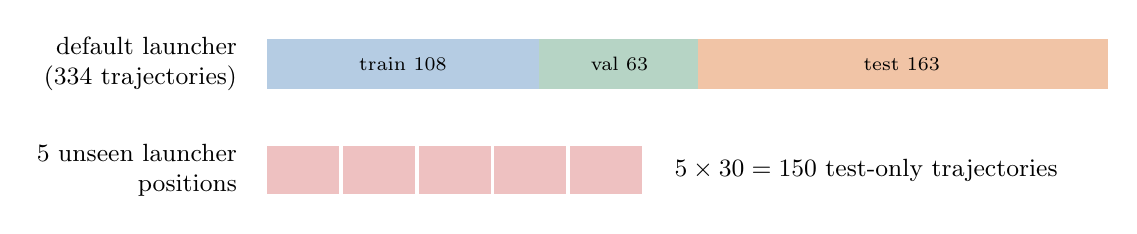
\begin{tikzpicture}[x=0.032cm,y=0.9cm]
\fill[cblue!35] (0,2.4) rectangle (108,3.1); \node[font=\scriptsize] at (54,2.75) {train 108};
\fill[cgreen!35] (108,2.4) rectangle (171,3.1); \node[font=\scriptsize] at (140,2.75) {val 63};
\fill[corange!40] (171,2.4) rectangle (334,3.1); \node[font=\scriptsize] at (252,2.75) {test 163};
\node[anchor=east,font=\small,align=right] at (-8,2.75) {default launcher\\ (334 trajectories)};
\foreach \i in {0,...,4} {\fill[cred!30,draw=white] (\i*30,0.9) rectangle (\i*30+29,1.6);}
\node[anchor=east,font=\small,align=right] at (-8,1.25) {5 unseen launcher\\ positions};
\node[anchor=west,font=\small] at (158,1.25) {$5\times30=150$ test-only trajectories};
\end{tikzpicture}
\caption{Data \textbf{(paper)}: default orientation 334 trajectories split 108 / 63 / 163; five unseen positions/orientations with 30 test trajectories each.}
\end{figure}
Launcher settings per trajectory, sampled uniformly \textbf{(paper)}: $s_\phi\in[0.4,0.6]$, $s_\theta\in[0.7,1.0]$; $s_{tl}\in[0.095,0.155]$ (default) or $[0.105,0.165]$ (unseen);
$s_{tr},s_b\in[0.135,0.195]$ (default) or $[0.145,0.205]$ (unseen). So the unseen sets also use slightly \emph{stronger} motor settings --- a real generalisation test.

\paragraph{Augmentation.} Each training trajectory is rotated about the vertical axis by a random angle $\phi_f\in[0,2\pi]$ around its lowest point; 19 rotated copies per trajectory are added (``augmented dataset'').
Physics does not depend on the compass direction, so this is free extra data in new directions.

\subsection{Evaluation protocol (4.2)}
\begin{itemize}
\item Filter until \textbf{one second before the end} of the trajectory, then predict the rest without measurements. For short trajectories, filter at least 10 measurements.
\item Error per trajectory = the \textbf{maximum} Euclidean distance over the \textbf{last five} prediction--measurement pairs.
\item Every method is trained \textbf{ten times independently}; plots show the spread over the ten models.
\end{itemize}

\subsection{Baselines (4.2)}
\begin{itemize}
\item \textbf{RSSM} (re-implementation of Hafner et al.\ 2019, ``PlaNet'' code): standard settings except ``free nats'' $=0.3$, chosen for minimal validation error; 100{,}000 training steps; optionally receives the launch information as an ``action'' input.
\item \textbf{TVAE} (G\'omez-Gonz\'alez et al.\ 2020, authors' code): model length 250 (longest trajectory has 235 steps); trained until the validation loss increases.
\end{itemize}

\subsection{Results (4.2, Fig.~5, Fig.~6, Fig.~S.1)}
\begin{itemize}
\item \textbf{EKF beats RSSM and TVAE in all settings} (default and unseen, with and without launch info). Fig.~5a switches from a linear to a log scale above 1 m because the black boxes' errors are so large.
\item \textbf{Augmentation is important} for the EKF to generalise to unseen launcher positions (``EKF w/o aug.'' is worse there).
\item \textbf{Launch information reduces the EKF error drastically}, on default and unseen positions (Fig.~5b, scale 0--0.4 m).
\item \textbf{Numbers in the text} (Fig.~6, unseen positions, with launch info, over 10 models): max error 0.393 m, \textbf{median 0.103 m}, min 0.006 m.
\item \textbf{All horizons} (Fig.~S.1, 150 unseen trajectories, 10 models each, median and 10--90\% band): the EKF is best for every horizon 0.1--1.0 s; launch info generally lowers the error.
\end{itemize}

\subsection{Spin evaluation (4.3, Eq.~8, Fig.~7)}
To check that the network's spin is physically meaningful, they build a simple spin model from the launcher geometry for a launcher shooting along $-y$:
\begin{eqbox}[Equation 8 (paper)]
\[
\ww_{\rightarrow-y}=\omega_{tl}\,\alpha\Big(\tfrac12,0,-\tfrac{\sqrt3}{2}\Big)^{\!\top}+\omega_{tr}\,\beta\Big(\tfrac12,0,\tfrac{\sqrt3}{2}\Big)^{\!\top}+\omega_b\,\gamma\,(-1,0,0)^\top .
\]
\textbf{Words:} each wheel adds spin proportional to its angular speed ($\omega_{tl},\omega_{tr},\omega_b$, measured, Fig.~4c), scaled by an unknown constant ($\alpha,\beta,\gamma$).
The bottom wheel spins the ball about $-x$; the top wheels' directions are that vector rotated by $120^\circ$ and $240^\circ$ about the $y$ axis (the wheels sit $120^\circ$ apart).
\end{eqbox}
Procedure: compute the network's canonical spin for each default test trajectory, rotate by $-90^\circ$ about $z$ (to the $-y$ direction), fit $\alpha,\beta,\gamma$ by least squares to Eq.~8.
Fig.~7: the two estimates \textbf{correlate highly} in all three axes $\Rightarrow$ the network's spin is plausible.

\paragraph{Spin only up to a scale.} In Eq.~1, $k_m$ and $\ww$ appear as a product, so $(2k_m,\ \ww/2)$ gives the same motion as $(k_m,\ww)$. Without extra physics the spin is known only up to a factor.
The true spin would be $\ww^*=k_m\ww/k_m^*$ with $k_m^*=C_m\rho Ar/(2m)$ for known mass, lift coefficient, radius, air density and cross-section \textbf{(paper)}.

\subsection{Return performance (4.4, Fig.~1, Fig.~S.2)}
The EKF estimates position, velocity and spin continuously; the learned model is simulated forward in a \textbf{receding horizon} scheme from the latest estimate; the predicted path gives an \textbf{interception point} (position and time) for the racket;
it is recomputed whenever the estimate improves. The arm is controlled by a learning-based iterative tracking controller (Ma et al.\ 2022).
\textbf{Result: 29 of 30 balls returned} with launch information; \textbf{26 of 30} without it (supplement S.2).
\begin{warn}[My comment: percentage slip]
The paper writes ``29/30 (97.7\%)''. But $29/30=96.7\%$. Quote the count, not the percentage.
\end{warn}

% =====================================================================
\section{Supplement S.3 --- initial and learned values, translated}
\subsection{Initial values (Table S.1)}
$\mathbf C$ starts as ``horizontal velocity unchanged, vertical velocity flips sign, spin unchanged'': $\mathbf C_0=\mathrm{diag}(1,1,-1,1,1,1)$ --- a perfectly elastic, frictionless bounce.
The table gives starting \emph{variances} (after softplus). I add the standard deviations to make them readable:
\begin{table}[htbp]
\centering\small\renewcommand{\arraystretch}{1.2}
\begin{tabular}{@{}lll@{}}
\toprule
Parameter & initial variance (paper) & standard deviation (mine)\\
\midrule
initial position $\splus{\boldsymbol\sigma_p}$ & $10^{-4}$ per axis & 1 cm\\
initial velocity $\splus{\boldsymbol\sigma_v}$ & $10^{-2}$ per axis & 0.1 m/s\\
initial spin $\splus{\boldsymbol\sigma_\omega},\splus{\boldsymbol\sigma_{\omega,\text{ai}}}$ & $1$ per axis & 1 rad/s\\
$\splus{\sigma_{a_d}},\splus{\sigma_{a_m}}$ & $10^{-2}$ & 0.1\\
camera $\splus{\boldsymbol\sigma_r}$ & $10^{-3}$ per axis & 3.2 cm\\
process, position $\splus{\boldsymbol\sigma_q[1{:}3]}$ & $10^{-4}$ & 1 cm per step\\
process, velocity $\splus{\boldsymbol\sigma_q[4{:}6]}$ & $10^{-2}$ & 0.1 m/s per step\\
process, spin $\splus{\boldsymbol\sigma_q[7{:}9]}$ & $10^{-3}$ & 0.03 rad/s per step\\
process, $a_d,a_m$ $\splus{\boldsymbol\sigma_q[10]},\splus{\boldsymbol\sigma_q[11]}$ & $10^{-2}$ & 0.1 per step\\
initial means $a_d,a_m$ & $\sqrt{0.1}$ each & $\Rightarrow k_d=k_m=0.1+0.05=0.15$\\
\bottomrule
\end{tabular}
\caption{Starting values. The initial spin variance is large on purpose: without launch info or after an impact, the spin is very uncertain (paper).}
\end{table}

\subsection{Learned values (Table S.2, one model with launch info, augmented data)}
\begin{table}[htbp]
\centering\small\renewcommand{\arraystretch}{1.2}
\resizebox{\textwidth}{!}{\begin{tabular}{@{}lll@{}}
\toprule
Parameter & learned value (paper) & meaning (mine)\\
\midrule
initial position var. $\splus{\boldsymbol\sigma_p}$ & $(1.38,1.63,1.00)\cdot10^{-6}$ & $\approx$1.2 mm: the first measurement is trusted\\
initial velocity var. $\splus{\boldsymbol\sigma_v}$ & $(0.12,0.14,0.09)$ & $\approx$0.35 m/s: finite difference of 2 points is rough\\
spin var.\ after impact $\splus{\boldsymbol\sigma_{\omega,\text{ai}}}$ & $(0.19,3.28,0.12)$ & mostly uncertain about spin around $y$\\
$\splus{\sigma_{a_d}}$, $\splus{\sigma_{a_m}}$ & $5.70\cdot10^{-6}$, $3.10\cdot10^{-3}$ & drag almost fixed; Magnus constant free-er\\
camera $\splus{\boldsymbol\sigma_r}$ & $(1.02,1.03,1.00)\cdot10^{-6}$ & $\approx$1 mm camera noise\\
process pos.\ $\splus{\boldsymbol\sigma_q[1{:}3]}$ & $(1.00,1.00,1.00)\cdot10^{-6}$ & 1 mm per step\\
process vel.\ $\splus{\boldsymbol\sigma_q[4{:}6]}$ & $(1.16,1.19,1.10)\cdot10^{-6}$ & 1 mm/s per step: physics trusted\\
process spin $\splus{\boldsymbol\sigma_q[7{:}9]}$ & $(1.73\cdot10^{-3},\,1.31\cdot10^{-3},\,1.00\cdot10^{-6})$ & spin about $x,y$ may drift\\
process $a_d$, $a_m$ & $1.16\cdot10^{-6}$, $1.30\cdot10^{-3}$ & drag constant; Magnus allowed to adapt\\
initial mean $a_d$ & $0.2168$ & $k_d=0.047+0.05\approx0.097$ /m\\
initial mean $a_m$ & $1.22\cdot10^{-5}$ & $k_m\approx\epsilon=0.05$ (at its floor)\\
\bottomrule
\end{tabular}}
\caption{Learned values (paper) with my interpretation. Several values ($10^{-6}$) sit exactly at the softplus floor, i.e.\ the optimiser pushed them as low as allowed.}
\end{table}

\begin{warn}[My comments on the learned values]
\begin{itemize}
\item The column header of Table S.2 says ``Initial value'' although the table holds learned values (a copy-paste slip).
\item $a_m$ collapsed to $\approx0$, so $k_m$ sits at $\epsilon=0.05$. This is the scale ambiguity in action: since $k_m$ and $\ww$ only appear as a product, the optimiser can put the size into $\ww$ (from the network) and leave $k_m$ at its floor.
\item Many variances at $10^{-6}$ (the floor) suggest the model is very confident in the physics; with real noise only $\approx$1 mm, this is plausible but means the floor itself may be limiting.
\end{itemize}
\end{warn}

\subsection{The learned bounce map (Eq.~S.1)}
\[
\mathbf C=\begin{pmatrix}\mathbf C_{vv}&\mathbf C_{v\omega}\\ \mathbf C_{\omega v}&\mathbf C_{\omega\omega}\end{pmatrix}=
\left(\begin{array}{rrr|rrr}
0.54&-0.01&-0.00&-0.01&0.12&0.01\\
0.01&0.55&0.00&-0.11&-0.01&-0.01\\
-0.01&-0.00&-0.92&0.01&0.00&0.00\\ \hline
0.19&-1.40&0.01&-0.20&0.09&-0.03\\
1.44&0.14&-0.03&-0.01&-0.12&-0.01\\
0.01&-0.05&0.15&0.05&-0.05&1.37
\end{array}\right)\quad\textbf{(paper)}
\]
\begin{itemize}
\item $\mathbf C_{vv}$ (velocity $\to$ velocity): horizontal speeds kept at $\approx$55\% (0.54, 0.55), vertical speed flips sign and keeps 92\% ($-0.92$, the vertical restitution). No mixing between axes.
\item $\mathbf C_{v\omega}$ (spin $\to$ velocity): spin about $y$ increases $v_x$ (0.12); spin about $x$ decreases $v_y$ ($-0.11$). This is the ``kick'' that spin gives at the bounce.
\item $\mathbf C_{\omega v}$ (velocity $\to$ spin): $-y$ velocity increases spin about $x$ ($-1.40$), $+x$ velocity increases spin about $y$ (1.44): the table's friction makes the ball start rolling. A downward $v_z$ reduces spin about $z$ (0.15).
\item $\mathbf C_{\omega\omega}$: the bottom-right entry 1.37 means spin about $z$ is \emph{amplified} by the bounce, which is physically odd. The authors suspect it cancels with the attenuation from $v_z$, and leave constraints (e.g.\ symmetry) and nonlinear impact models to future work.
\end{itemize}

% =====================================================================
\section{Conclusion of the paper (Section 5)}
A physically grounded aerodynamic model (drag, Magnus) inside an EKF, with parameters fitted on offline data, gives accurate filtering and prediction, and ``no tedious tuning of initial, transition, and observation covariances is required''.
A neural model for the initial spin from launch information drastically improves long-term prediction. Positions alone are insufficient to estimate spin (agreeing with earlier work). Future work: use the racket movement to estimate spin.

% =====================================================================
\section{Critical reading}
\begin{idea}[Strengths]
\begin{enumerate}
\item Interpretable: every learned number has a physical meaning ($k_d$, $\mathbf C$, noise levels) and can be checked (they did, for $\mathbf C$ and spin).
\item No hand-tuning of covariances: one principled objective learns them all.
\item Data-efficient: 108 training trajectories (plus rotations) suffice, because physics carries most of the knowledge.
\item Careful implementation: impact time inside a step, full Jacobian through the impact timing (supplement S.4), missing measurements handled.
\item Tested on a real robot, with and without launch info (29/30 vs 26/30).
\end{enumerate}
\end{idea}
\begin{warn}[Weak points and things to check]
\begin{enumerate}
\item \textbf{Only black-box rivals.} No comparison with a classic hand-tuned EKF/UKF using the same physics. The paper shows ``physics + learning beats pure learning'', not ``learned covariances beat carefully tuned ones''.
\item \textbf{Demanding, unusual metric}: maximum of the last five errors after a fixed 1 s prediction --- a worst-case-near-the-end measure, not an average.
\item \textbf{Mostly plots}: exact numbers only for Fig.~6 (max / median / min) and the return counts.
\item \textbf{Small slips}: 29/30 printed as 97.7\% (is 96.7\%); Table S.2 header says ``initial''; $\epsilon$ missing in S.3/S.4; likelihood written with the 11-dim mean/covariance instead of $\mathbf H\mmu$, $\mathbf S$.
\item \textbf{Linear bounce map} with an unphysical entry (spin about $z$ amplified).
\item \textbf{Impact time with gravity only} (drag and Magnus ignored inside $\Delta_{\text{imp}}$) --- fine for 5.56 ms steps, but an approximation.
\item \textbf{Narrow world}: one table, one ball type, one lab launcher; launcher-based spin needs known launcher settings, which do not exist in a match.
\end{enumerate}
\end{warn}
\textbf{Correction to the earlier short guide:} it said the paper does not discuss how the EKF linearises at the bounce. The supplement (S.4) does: it derives the full Jacobian through the impact, including the dependence of the impact time on the state.

% =====================================================================
\section{What we take for our project (state on 2026-10-31)}
\subsection{Mapping}
\begin{table}[htbp]
\centering\small\renewcommand{\arraystretch}{1.25}
\begin{tabularx}{\textwidth}{@{}p{3.2cm}XX@{}}
\toprule
 & Paper 03 & Our project \\
\midrule
Motion between contacts & gravity + drag + Magnus, 3D & planar sliding friction: deceleration $\mu$ opposite to $\vv$ \\
Constants in the state & $a_d,a_m$ (air) & $\mu$ (friction), later $E$ (restitution) \\
Contacts & table, learned $6\times6$ map & 4 walls + static arm base box, restitution $E$ \\
Hidden quantity & spin & none (no spin), but $\mu$ and $E$ unknown per launch \\
Extra info at launch & launcher settings $\to$ spin & none given to the estimator \\
Sensor & 4 RGB cameras, 180 Hz, $\approx$1 mm & 1 depth camera, 60 Hz, 3 m, 8 sensor conditions (up to $\approx$33 mm depth noise) \\
Data & 108 / 63 / 163 (+150 unseen) & 350 / 75 / 75 launches (\texttt{split\_500.json}) \\
\bottomrule
\end{tabularx}
\end{table}

\subsection{Why this paper targets our main problem}
Our best baseline ekf19b uses one fixed $\mu=0.85$ and $E=0.725$ for every launch. The oracle (true $\mu$, $E$) is about $3\times$ better at 0.5 s in every sensor condition.
A check on all 500 launches (\texttt{experiments/step\_1a\_mu\_vs\_e\_gap.py}) splits the gap (0.5 s error, RMS / median, mm):
\begin{center}\small
\begin{tabular}{lcc}
\toprule
EKF knows & ideal & all\_real\\
\midrule
nothing (= ekf19b) & 73 / 47 & 99 / 69\\
true $\mu$ only & 50 / 6 & 64 / 20\\
true $E$ only & 55 / 43 & 81 / 64\\
both (= oracle) & 23 / 5 & 36 / 16\\
\bottomrule
\end{tabular}
\end{center}
$\Rightarrow$ $\mu$ explains almost all of the \emph{typical} error; $E$ matters for the bounce \emph{tail}. Paper 03's idea --- unknown constants inside the state --- is exactly what is needed for $\mu$.

\subsection{Proposed design: ekf-$\mu$ (step 1.2, to be decided)}
\begin{ours}[ekf-$\mu$ in equations]
\textbf{State:} $\zz=(x,y,v_x,v_y,\mu)^\top$. To keep $\mu$ positive one can use $\mu=a^2+\epsilon$ (paper's trick) or softplus.\\
\textbf{Model per sub-step $h$} (as in \texttt{estimators/model.py}): if $\mu h<\|\vv\|$: $\vv'=\vv-h\mu\hat\vv$, else $\vv'=\mathbf 0$; $\pp'=\pp+h\vv'$; $\mu'=\mu$; then wall / arm-box reflection with $E$.\\
\textbf{Jacobian (new parts):}
\[
\frac{\partial\vv'}{\partial\vv}=\mathbf I-\frac{h\mu}{\|\vv\|}\big(\mathbf I-\hat\vv\hat\vv^\top\big),\qquad\frac{\partial\vv'}{\partial\mu}=-h\,\hat\vv,\qquad\frac{\partial\pp'}{\partial\mu}=-h^2\hat\vv,\qquad\frac{\partial\mu'}{\partial\mu}=1 .
\]
\textbf{Measurement:} $\mathbf H=[\mathbf I_2,\ \mathbf 0_{2\times3}]$ (camera gives $x,y$).\\
\textbf{Learned by maximum likelihood on the 350 train launches} (Eq.~7 with $\mathbf S=\mathbf H\SSigma\mathbf H^\top+\mathbf R$): measurement variance $\sigma_r^2$, process noise on velocity $q$, random-walk noise on $\mu$ $q_\mu$,
initial mean $\mu_0$ and variance $\sigma_{\mu,0}^2$, initial velocity variance. About 6 numbers per sensor condition.\\
\textbf{Evaluate on TEST:} ekf19b+stale vs ekf-$\mu$ (hand-tuned) vs ekf-$\mu$ (learned) vs oracle, 8 conditions, RMS / median / p95, plus how fast $\hat\mu\to\mu$.
\end{ours}
\textbf{Why $\mu$ is observable:} friction changes the speed steadily, so after a few frames the deceleration shows in the positions ($\Delta x\approx\tfrac12\mu t^2$). With 60 Hz and mm-level noise it should be identified within a fraction of a second for fast balls; slow balls stop quickly and give less information.
$E$ is observable only at a bounce, which is why it is a separate step (paper 18).

% =====================================================================
\section{Test yourself (with answers)}
\begin{enumerate}
\item \emph{What makes the model ``gray-box''?} Physics structure (Eqs.~1--5) is fixed; only numbers (noise, initial beliefs, constants, $\mathbf C$, spin net) are learned.
\item \emph{Why are $a_d,a_m$ in the state?} So the filter can estimate the air constants per ball while it flies, instead of using one fixed value.
\item \emph{Why $k_d=a_d^2+\epsilon$?} Keeps $k_d\geq0.05>0$ without constraints and stabilises training.
\item \emph{How does the filter correct spin if spin is never measured?} Through the covariance links between spin and future positions; the Kalman gain spreads the position surprise to spin.
\item \emph{What does Eq.~7 add up?} The log probability the filter gave to each new measurement before seeing it: $\log\mathcal N(\mm_n;\mathbf H\mmu,\mathbf H\SSigma\mathbf H^\top+\mathbf R)$.
\item \emph{Why do both terms of the Gaussian log density matter?} The surprise term punishes being wrong, the log-determinant term punishes claiming too much uncertainty; together they calibrate the noise levels.
\item \emph{Why is $\Delta_{\text{imp}}$ differentiated?} Because the bounce time depends on height and vertical speed; ignoring it gives a wrong Jacobian at bounce steps.
\item \emph{What does $-0.92$ in $\mathbf C$ mean?} The vertical speed flips sign and keeps 92\% of its size at the bounce.
\item \emph{Why can spin be found only up to a scale?} $k_m$ and $\ww$ appear only as a product $k_m\ww$.
\item \emph{What is the 1 s median error on unseen positions?} 10.3 cm (with launch info).
\item \emph{How many balls did the robot return?} 29/30 with launch info, 26/30 without (the printed 97.7\% should be 96.7\%).
\item \emph{What is the main thing we copy?} Put the unknown per-launch constant ($\mu$) into the EKF state and learn the filter's noise numbers by maximum likelihood on training launches.
\end{enumerate}

% =====================================================================
\section{Equation cheat sheet}
\begin{eqbox}[All equations on one page]
\textbf{Flight:} $\dot\vv=-k_d\|\vv\|\vv+k_m(\ww\times\vv)+\mathbf g$, \ $\mathbf g=(0,0,-9.802)$.\qquad \textbf{Impact:} $(\vv^+,\ww^+)=\mathbf C(\vv^-,\ww^-)$.\\
\textbf{State:} $\zz=(\pp,\vv,\ww,a_d,a_m)\in\mathbb R^{11}$, $k_{d,m}=a_{d,m}^2+0.05$, $\Delta T=1/180$ s.\\
\textbf{Euler:} $\pp'=\pp+\Delta_t\vv$, $\vv'=\vv+\Delta_t(\dots)$, $\ww,a_d,a_m$ constant.\\
\textbf{Impact time:} $\Delta_{\text{imp}}=-(v_z+\sqrt{v_z^2+2g_zh})/g_z$, $h=-((p_z-r)-z_{\text{table}})$.\\
\textbf{Noise:} $\mathbf Q=\mathrm{diag}(\splus{\boldsymbol\sigma_q})$, $\mathbf R=\mathrm{diag}(\splus{\boldsymbol\sigma_r})$, $\splus{x}=\log(1+e^x)+10^{-6}$.\\
\textbf{Predict:} $\mmu^-=g(\mmu)$, $\SSigma^-=\mathbf J\SSigma\mathbf J^\top+\mathbf Q$.\\
\textbf{Correct:} $\mathbf S=\mathbf H\SSigma^-\mathbf H^\top+\mathbf R$, $\mathbf K=\SSigma^-\mathbf H^\top\mathbf S^{-1}$, $\mmu=\mmu^-+\mathbf K(\mm-\mathbf H\mmu^-)$, $\SSigma=(\mathbf I-\mathbf K\mathbf H)\SSigma^-$.\\
\textbf{Learning:} maximise $\sum_{n=3}^{50}\log\mathcal N(\mm_n;\mathbf H\mmu_n^-,\mathbf S_n)$ over chunks of 50; Adam, lr $5\cdot10^{-3}$, batch 64.\\
\textbf{Jacobian pieces:} $\partial(\|\vv\|\vv)/\partial\vv=\|\vv\|\mathbf I+\vv\vv^\top/\|\vv\|$; $\partial(\ww\times\vv)/\partial\vv=[\ww]_\times$; $\partial(\ww\times\vv)/\partial\ww=-[\vv]_\times$.
\end{eqbox}

\section{Where each part is in the paper}
\begin{center}\small
\begin{tabular}{ll}
\toprule
Topic & Location in the paper\\
\midrule
Contributions & Abstract, Section 1\\
Related work (box types, table tennis) & Section 2, 2.1\\
Flight ODE, impact map & Section 3.1, Eqs.~1--2\\
State, Euler step, impact time, joint model & Section 3.2, Eqs.~3--5\\
Noise, EKF, initialisation, spin from launcher, $\Psi$ & Section 3.3, Eq.~6\\
Learning objective, chunks, Adam & Section 3.3 (``Learning''), Eq.~7\\
Set-up, launcher, data, augmentation & Sections 4.1, 4.1.1, 4.1.2; Figs.~2--4\\
Protocol, baselines, results & Section 4.2; Figs.~5--6\\
Spin plausibility & Section 4.3; Eq.~8, Fig.~7\\
Robot return & Section 4.4; Fig.~1\\
All horizons; failed returns & Supplement S.1 (Fig.~S.1), S.2 (Fig.~S.2)\\
Initial / learned values, $\mathbf C$, spin network & Supplement S.3 (Tables S.1, S.2, Eq.~S.1, S.3.3)\\
Jacobians incl.\ impact & Supplement S.4 (Eqs.~S.2--S.7)\\
\bottomrule
\end{tabular}
\end{center}

\end{document}
